\section{Primary keys, Surrogate and Natural keys}
\begin{itemize}
    \item In every table of a relational database you have rows and columns, columns denote specific attributes, and rows denote each entry or object.
    \item Each table needs to have a \emph{primary key} attribute. In the above example the student id would be the primary key because it uniquely identifies each student. This allows us to have repeated names, notice that student number 2 and 4 have the same name and major, the primary key differentiates them and therefore there is no problem.
    \item A primary key can be anything such as a string, a number or character, the only requisite is that they are unique in the table.
    \item Example:
        \begin{figure}[H]
            \centering
            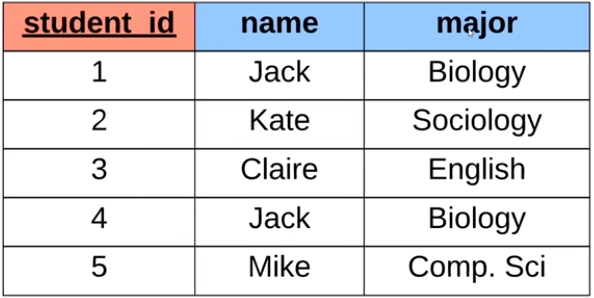
\includegraphics[width=0.4\textwidth]{./figs/example.png}
        % 	\caption{\href{}{source}}
        \end{figure}
\end{itemize}

%----------------------------------------------------------------------------------------
\subsection{Another example}
\begin{itemize}
    \item Example:
        \begin{figure}[H]
            \centering  
            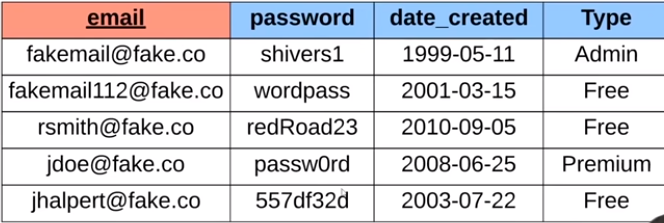
\includegraphics[width=0.4\textwidth]{./figs/example1.png}
        % 	\caption{\href{}{source}}
        \end{figure}

    \item Notice the emp\_id, this is a primary key. In this particular example it is a Surrogate Key or a key that has no mapping in the real world: 
        \begin{figure}[H]
            \centering
            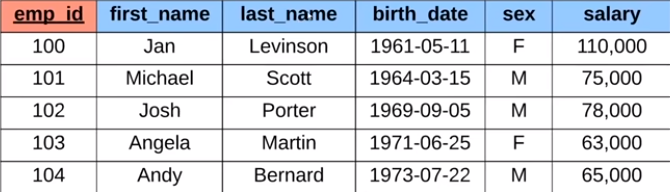
\includegraphics[width=0.4\textwidth]{./figs/example2.png}
        % 	\caption{\href{}{source}}
        \end{figure}

    \item Notice here the primary key is the social security number. This is called a natural key, this is a key that has a purpose or a mapping in the real world.
        \begin{figure}[H]
            \centering
            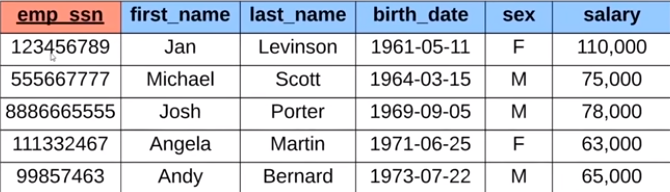
\includegraphics[width=0.4\textwidth]{./figs/example3.png}
        % 	\caption{\href{}{source}}
        \end{figure}
\end{itemize}

\subsection{Difference between Surrogate and natural keys}
\begin{itemize}
    \item Both are types of primary keys.
    \item A surrogate key serves only to identify a particular object inside a database such as an id or a hash, this key has no significance nor mapping outside the database.
    \item A natural key is a registration of an individual object using natural attributes, such as a social security number, this type of key has significance outside and inside the database.
\end{itemize}


%----------------------------------------------------------------------------------------
\section{Foreign Keys and composite keys}
\begin{itemize}
    \item An attribute that you can store that allow the object to be linked to another database table.
    \item For example in the below figure suppose that we have employees and in the company we have different branches, and we want to store the information, in this case we can store that using a foreign key: 
        \begin{figure}[H]
            \centering
            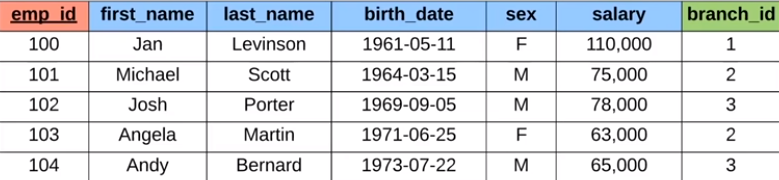
\includegraphics[width=0.4\textwidth]{./figs/example4_1.png}
            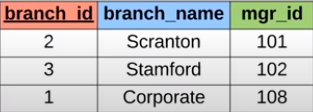
\includegraphics[width=0.4\textwidth]{./figs/example4_2.png}
        % 	\caption{\href{}{source}}
        \end{figure}
        \begin{itemize}
            \item In the above, we can see that for example Josh Porter belongs to the third branch, we can look up what is the third branch, in this case in another table, we quickly see that the third branch matches up to the Stamford branch.
            \item Notice how the foreign key ``branch\_id''is the primary key of the Branch dable.
        \end{itemize}
        
    \item A foreign key is a primary key inside another table.
    \item It is basically a way to define relationships with other tables.
    \item You can have multiple foreign keys:
        \begin{figure}[H]
            \centering
            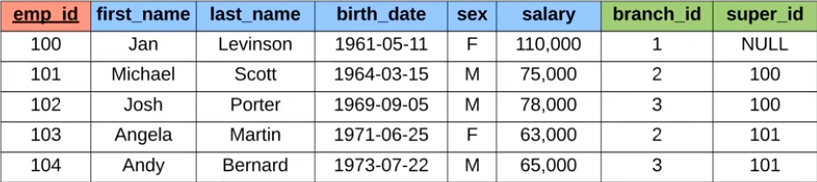
\includegraphics[width=0.4\textwidth]{./figs/example5.png}
        % 	\caption{\href{}{source}}
        \end{figure}
        \begin{itemize}
            \item In the above figure, take for example, Angela Martin has the supervisor id=101, this means that whoever has the id 101 is Angela's supervisor, in this case id 101 is Michael Scott. Michael Scott's supervisor is Jan (id=100), and Jan has no supervisor.
        \end{itemize}
    
    \item Taking the same example, lets add another foreign key that denotes who the suppliers are for each branch:
        \begin{figure}[H]
            \centering
            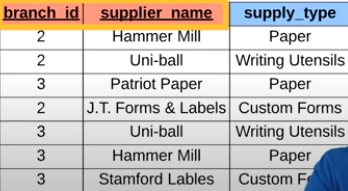
\includegraphics[width=0.4\textwidth]{./figs/example6.png}
        % 	\caption{\href{}{source}}
        \end{figure}
        \begin{itemize}
            \item In this case we use a composite key, composite keys are keys that only makes sense in groups. For example the above only makes sense if we say Hammer Mill supplies branch 2, even though 2 is repeated three times and Hammer Mill is repeated twice.
            \item We can say ``Hammer Mill supplies Paper to branch 2''.
            \item Composite keys are when you define the combination of two columns to be a primary key, which is to say the columns by themselves have repeated values but when they are in combination they do not repeat.
            \item This is why we've marked in orange (primary key) two columns.
        \end{itemize}
    
    \item Suppose we have another database of clients and another database of sales:
        \begin{figure}[H]
            \centering
            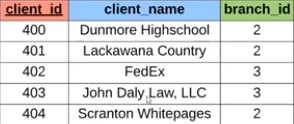
\includegraphics[width=0.4\textwidth]{./figs/example7.png}
            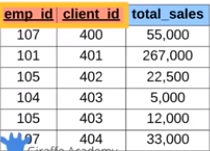
\includegraphics[width=0.4\textwidth]{./figs/example8.png}
        % 	\caption{\href{}{source}}
        \end{figure}
        \begin{itemize}
            \item Notice in this case emp\_id and client\_id are composite primary keys and at the same time they are foreign keys.
            \item We can see that we can calculate how much an employee has sold for example.
        \end{itemize}
    
    \item Notice as your databases get more and more complex you can split the database up in to multiple databases and establish a relationship between them using composite keys or foreign keys.
\end{itemize}

